\documentclass{article}

\usepackage{graphicx}
\usepackage{physics}
\usepackage{subcaption}
\usepackage{hyperref}
\usepackage{float}

\usepackage[left=2.5cm, right=2.5cm, top=2.5cm, bottom=2.5cm]{geometry}
\setlength{\parindent}{0em}
\setlength{\parskip}{0.8em}

\usepackage{caption}
\captionsetup{width=.9\textwidth}

\usepackage{biblatex}
\addbibresource{report.bib}

\title{Exam, TFY4235 Computational physics}
\author{Number}
\vspace{-8ex}
\date{}


\begin{document}
    \maketitle
    \section*{Introduction}
    SIR, and the more advanced SEIIaR, are mathematical models that aim to capture how pandemics spread throughout a simulation.
    This paper documents the implementation and results of the simulation of these models in Python, as described in \cite{exam}.

    \section*{Implementation}
    All the different models used in this text follow the same basic form. 
    The goal is to find $x(t)$, given initial conditions $x(t_0)$, and a equation of the form
    \begin{equation*}
        f(x(t); \mathrm{args}) = \dv{x(t)}{t}.
    \end{equation*}
    In the first part, $x = (S, I, R)$, while later $x = (S_{ij}, E_{ij}, I_{ij}, Ia_{ij}, R_{ij})$ where $(ij)$ are different population groups. 
    This is accomplished using function \verb|integrate| in \verb|utilities.py|. 
    It takes as arguments the initial conditions \verb|x0|, the functions \verb|f| and \verb|step|, the list \verb|args| as well as the time step \verb|dt| and total time \verb|T| to simulate. 
    It then creates a discrete approximation of $x(t)$ by taking time steps given by the function \verb|step|. 
    \verb|step| is the particular \emph{scheme} used, for example Runge-Kutta (4,5), while \verb|f| defines the system. 


    The equations that give the asymptotic behavior are both of the type $x = f(x)$, and can thus be approximated by recursion, given that they converge. 
    For $\mathcal{R}_0$ close to one, they converge increasingly slowly, and the program may reach maximum recursion depth. 
    For the parameters in this exercise, however, this was not a problem

    \section*{Results}
    \subsection*{Deterministic SIR model}
    The first model is the deterministic SIR model, given by a set of coupled ODEs \cite{exam}. 
    In this text, the Runge-Kutta (4, 5) scheme was used, as it is both a simple yet precise scheme.
    \autoref{SIR} demonstrates that $S$ and $R$ approaches the expected asymptotes, and that $I$ grows exponentially in the beginning. 

    \begin{figure}
        \centering
        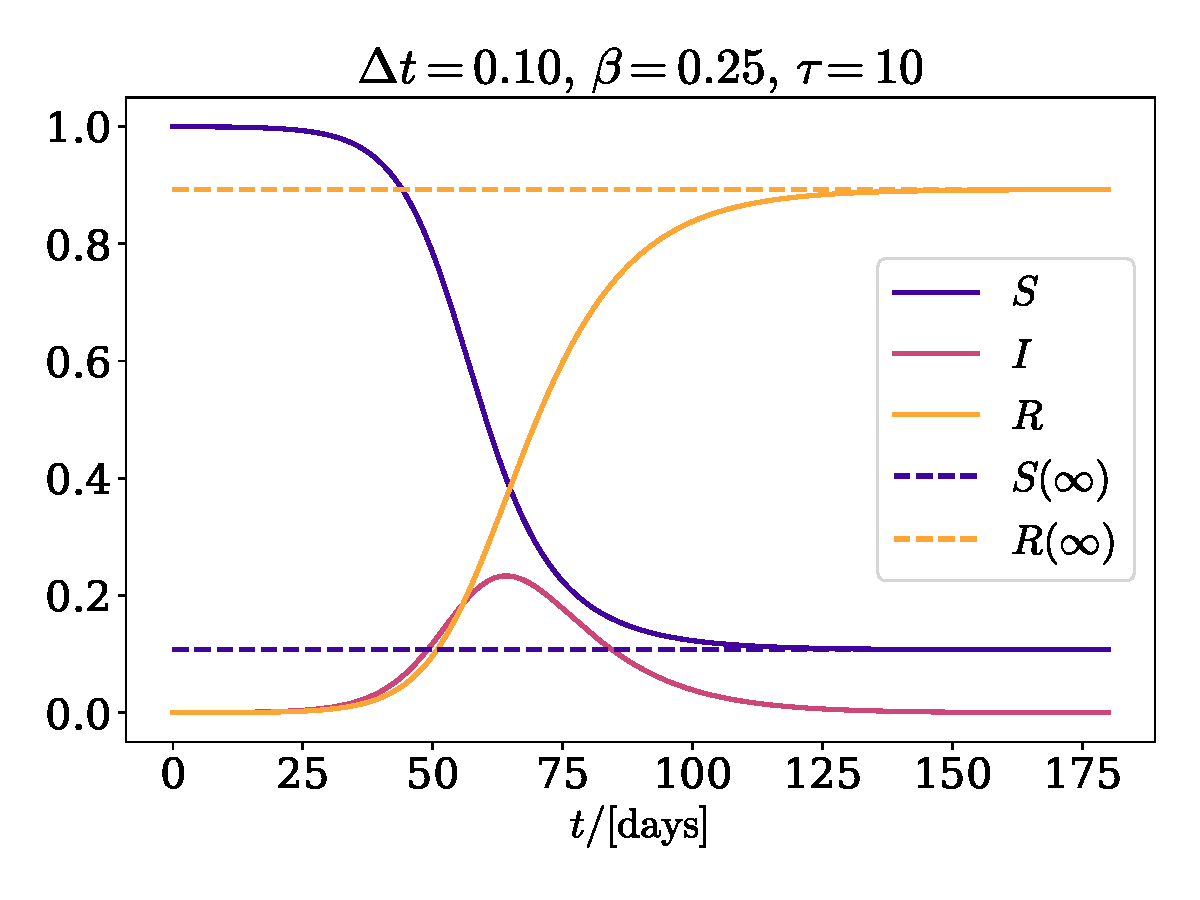
\includegraphics[width=.4\textwidth]{../plots/2A/TestSIR}
        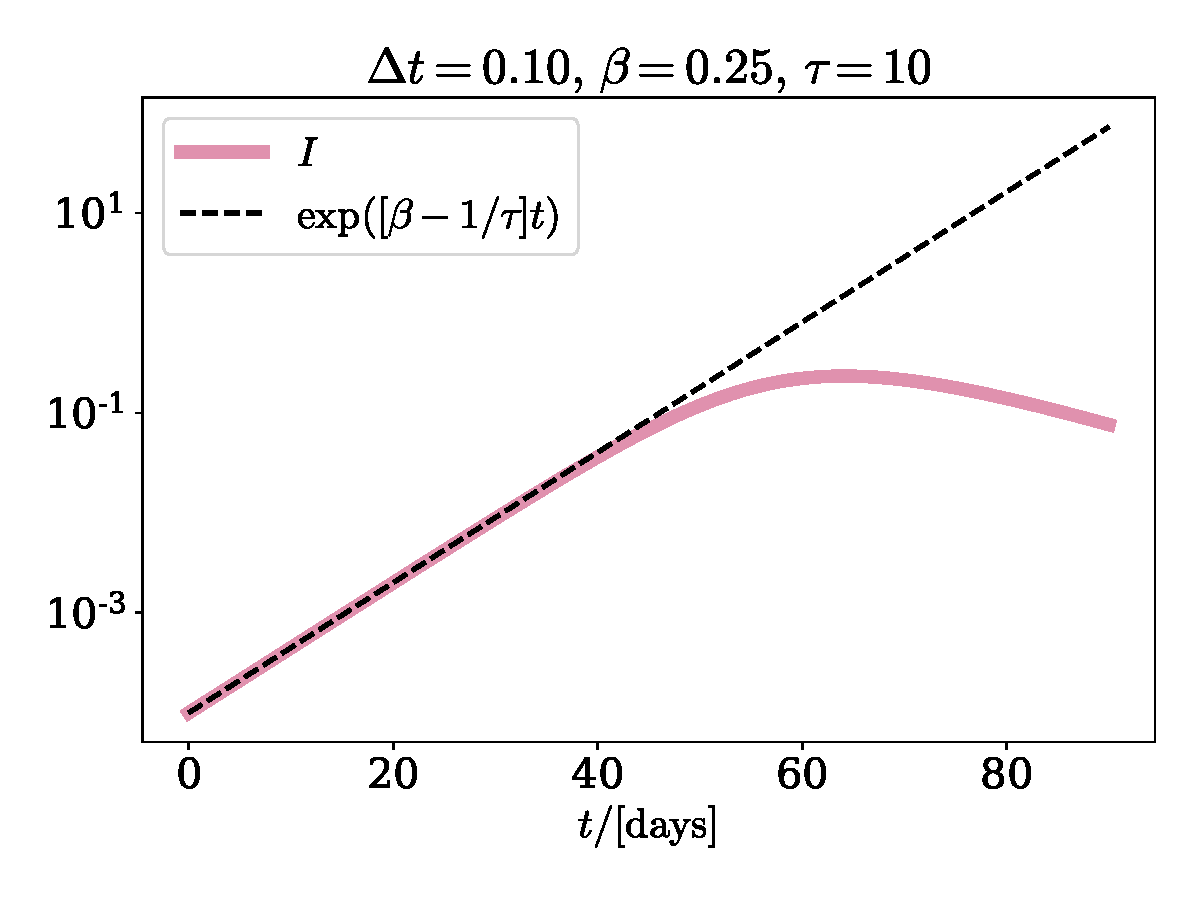
\includegraphics[width=.4\textwidth]{../plots/2A/TestI}
        \caption{On the left, the fraction of the population that is in each group, over time. The plot on the right shows how the infection spreads exponentially in the begining}
        \label{SIR}
    \end{figure}

    \printbibliography
\end{document}